\section{Access Control Hardware/Software Implementation}
\label{sec:ACD_implementation}

Implementation of ACD were performed with use of TinkerCAD that provided GUI for implementation of a circuit that contains an Ardruino board, breadboard, PIR motion sensor, LEDs, pushbuttons, resistors, and wiring. System runs on power of 5V, first thing that was done is connecting two wires for ground and power from Ardruino board to the breadboard. Further PIR – sensor was connected to the system as well, three wires in total two of them for power and grounding. Last one is providing signal and was connected to board at port 11.
\newline

\begin{figure}[h]
  \centering
  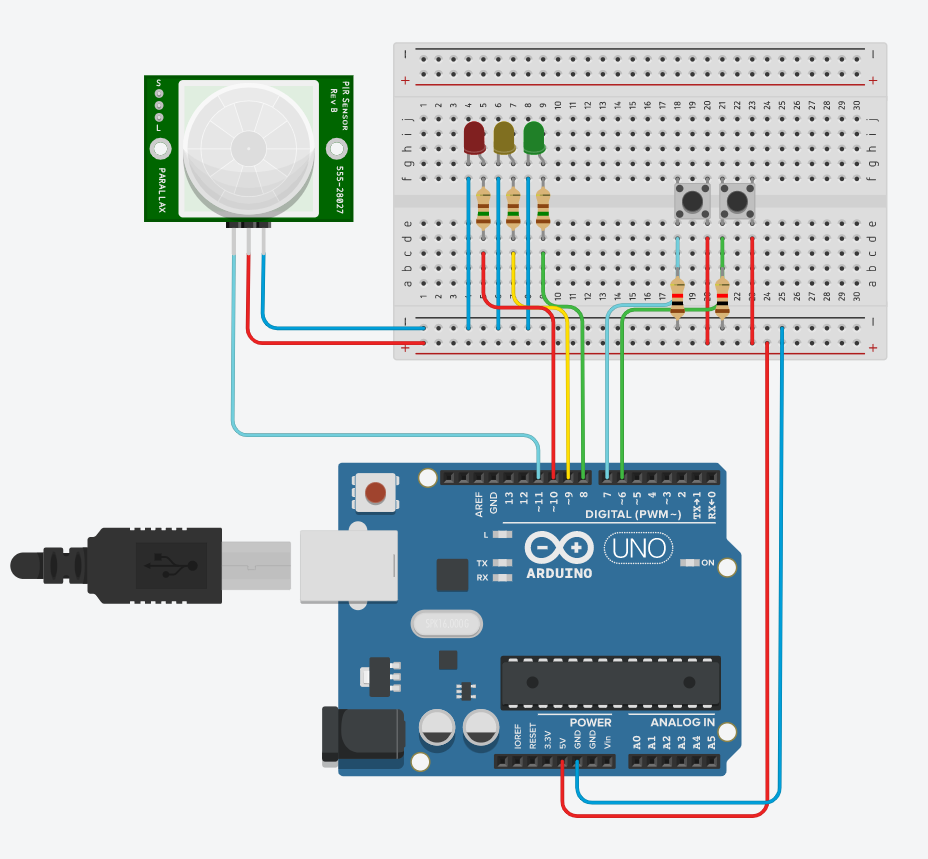
\includegraphics[scale=0.5]{figs/ACD_circut.png}
  \caption{TinkerCAD circuit design of access control device}
  \label{fig:framework}
\end{figure}
 
For the input of access code, system uses two pushbuttons that has two signal wires connected directly to the Ardruino board, two resistors that is used for grounding. And two wires that is providing power to the push buttons. Last step was to connect the LED bulbs, these are used to display different states of the system. As well as light up when input from the pushbuttons is registered and when the access code from input is incorrect. 
\newline

Red LED bulb is used to indicate incorrect access code setting state of system to locked. As well as locked state that is also initial state. Yellow LED bulb is indicating waiting state of the system, and blink during incoming input on-click from the pushbuttons. Green LED bulb is indicating unlock state for the system. All three LED bulbs are connected with one wire each for grounding, and one wire and resistor each for input signal from the board. Red LED is connected to port 10, yellow led is connected to port 9 and green LED is connected to port 8 at Ardruino board. 

Software implementation of ACD were performed and written using Ardruino version of C++ file format “*.ino” that stand for ending of Ardruino. First part of code is running setup(), where first method that is getting used Serial.begin(9600) method to establish serial communication between Ardruino and another device in this case is our computer. 9600 is the baud rate simply explained this number needs to match on both devices, to be able to send anything over serial. Further we define the pins that is used for input and output on the Ardruino board. 
\newline

After setup() method, we define variables and constants (cannot be modified). For this implementation, the correct access code is hardcoded. States are defined as constants and are not supposed to be changed, the same applies to access code.
\newline

Key part in the code is the method loop() where most of the functionality is taking place. Method is constantly getting called on while simulation is running. States of the system is implemented with use of a switch, where states are represented as cases. The PIR – sensor and the pushbuttons are called with method digitalRead(port number) inside of the loop. Since system needs to constantly monitor if there has been any input on those.  
\newline

There’re three cases that is implemented inside the loop, it is the same ones that is mentioned above locked, waiting and unlock. Logic behind case locked, is that if sensor has been triggered. And there has not been registered a movement before, then system goes over in waiting state. In waiting state there’s several conditions, first one is timer condition. Which sets system in locked state after some time without input. Second and third state is checking for input from pushbuttons and makes the yellow LED blink at push. Input from pushbuttons is padded to string named “current”, that represents input access code. Last two cases checks if the input access code if there’s any, matches the hardcoded valid access code. If the input access code matches hardcoded, system is set in unlocked state. If not, it’s set to locked. 
\newline

For the case unlocked, there’s implemented a timer that after some time in unlocked state. Puts system state back to locked. 
